\chapter{Fundamentação teórica}

\section{Treinamento de modelos de aprendizado de máquina}

O processo de treinamento de modelos de aprendizado de máquina nada mais é do que uma variação específica do processo padrão de mineração de dados, que consiste no ato de utilizar algoritmos para extrair informações relevantes de um banco de dados \cite{data-mining}.

Este processo já possui uma forma bem definida e aceita conhecida como CRISP-DM (\textit{Cross-Industry Standard Process for Data Mining}) \cite{crisp-dm}. 

O treinamento de modelos de aprendizado de máquina se enquadra como um processo de mineração de dados, pois nada mais é do que encontrar um modelo que, de alguma forma, represente o relacionamento entre diferentes aspectos do conjunto de dados. O modelo, nesse caso, representa a informação que se deseja extrair dos dados.

Um bom modelo descreverá com precisão o relacionamento entre os aspectos desejados do conjunto de dados e será portanto útil para extrair novas informações de novos dados.

\subsection{Etapas do padrão CRISP-DM}

O padrão CRISP-DM nada mais é que uma sequência de etapas a partir das quais é possível extrair informações úteis de um banco de dados, sendo que cada etapa é definida por tarefas e um resultado esperado.

As etapas são:

\begin{enumerate}
    \item \textbf{Entendimento do problema} \\
    A primeira fase consiste em entender as características do problema e os requisitos da solução, criando assim uma definição de problema de mineração de dados e um plano preliminar para atingir os objetivos \cite{crisp-dm}.
    \item \textbf{Entendimento dos dados} \\
    A fase seguinte envolve se familiarizar com os dados à disposição. Isso envolve descobrir \textit{insights} iniciais nos dados, detectar problemas de qualidade dos dados e identificar subsets interessantes \cite{crisp-dm}.
    \item \textbf{Preparação dos dados} \\
    Essa etapa consiste nas atividades necessárias para construir o \textit{dataset} final que será utilizado a partir dos dados brutos. Pode envilver diversas tarefas como limpeza dos dados, seleção de atributos relevantes e transformação dos dados \cite{crisp-dm}.
    \item \textbf{Modelagem} \\
    A modelagem envolve selecionar, aplicar e calibrar técnicas diversas de modelagem, buscando encontrar um modelo ótimo para o problema que se deseja resolver \cite{crisp-dm}.
    \item \textbf{Avaliação} \\
    Após chegar em um ou mais modelos que aparentam ser apropriados, uma avaliação final deles deve ser feita para concluir se atendem aos requisitos de negócio. Ao final dessa avaliação deve-se chegar em uma conclusão relativa ao uso ou não de cada modelo para o objetivo final \cite{crisp-dm}.
    \item \textbf{\textit{Deployment}} \\
    Por fim, a última etapa é o momento em que o conhecimento obtido é preparado para uso pelo cliente do projeto. Essa preparação depende muito dos requisitos, podendo ser em forma de um relatório ou de um sistema automatizado de mineração de dados \cite{crisp-dm}.
\end{enumerate}

A figura \ref{fig:crisp} mostra um diagrama do processo e demonstra como algumas das etapas possuem uma relação de troca, de forma que o conhecimento ou os desafios encontrados em uma dada etapa podem fazer com que seja necessário voltar para uma etapa anterior.

\begin{figure}[H]
    \centering
    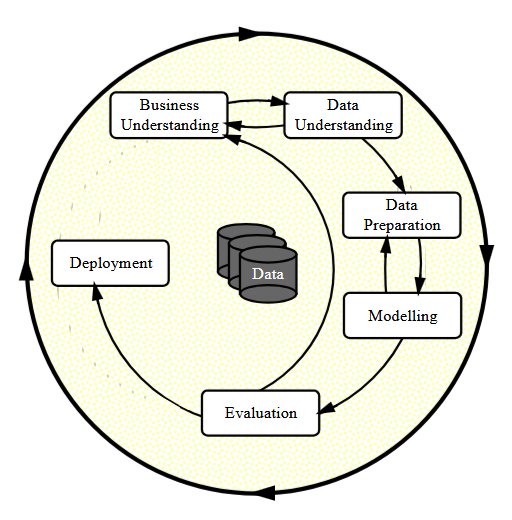
\includegraphics[width=0.5\linewidth]{images/crisp.png}
    \caption{Fases do processo CRISP-DM \cite{crisp-dm}}
    \label{fig:crisp}
\end{figure}

\section{Redes Neurais Convolucionais}

A eficácia de redes neurais convolucionais (CNNs) para tarefas de classificação e segmentação de imagens já é comprovada \cite{imagenet-cnn}, sendo uma solução amplamente utilizada em diversas aplicações.

Essa modalidade de rede neural possui como característica as camadas convolucionais, que possui vantagens em relação as camadas \textit{fully connected} tradicionais para terefas de interpretação de imagens ou mesmo de sinais \cite{cnn}.

A limitação das camadas \textit{fully connected} para esse tipo de tarefa se dá pelo fato de que esse tipo de camada produz sua saída com base no relacionamento entre todos os \textit{inputs} da camada uns com os outros. Isso é ótimo para achar relações entre diferentes atributos quando se trabalha com dados tabulares, por exemplo, mas não é tão bom para encontrar características específicas que podem estar localizadas em diferentes partes de uma imagem.

Para esse tipo de tarefa as camadas convolucionais são mais apropriadas, pois utilizam conectividade local e compartilhamento de pesos, reduzindo drasticamente a quantidade de parâmetros necessários para se ter um resultado satistaftório.

A camada convolucional funciona deslizando pelo \textit{input} um filtro chamado \textit{kernel}, que nada mais é do que uma matriz de pesos de dimensão pequena, como 3x3 ou 5x5. Em cada posição do \textit{kernel} é então feita uma transformação linear de um conjunto local de valores utilizando os pesos do \textit{kernel}. 

Fazendo isso em todo o \textit{input} obtêm-se um mapa de características, que destaca padrões identificados em cada parte do \textit{input}. Esse mapa de características pode então ser alimentado para outra camada convolucional e assim por diante. Além disso, para cada \textit{input} pode-se (e deve-se) ter múltiplos \textit{kernels}, de forma a ferar múltiplos mapas de características em cada camada, cada um destacando aspectos distintos do \textit{input}. A imagem \ref{fig:convolution} exemplifica o funcionamento da camada convolucional.

A equação da convolução 2D discreta utilizada nas camadas convolucionais para imagens é:

\begin{equation}
    (I * K)(x, y) = \sum_{i} \sum_{j} I(x+i, y+j) \cdot K(i, j)
\end{equation}

Sendo que $I$ é a imagem e $K$ é o \textit{kernel}.

\begin{figure}[H]
    \centering
    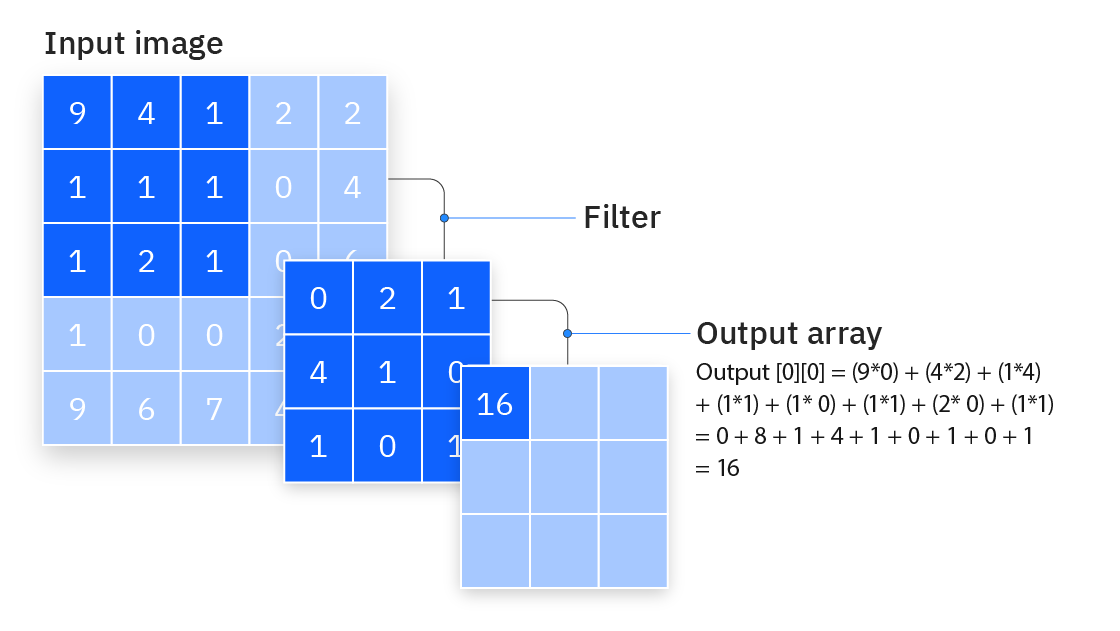
\includegraphics[width=0.8\linewidth]{images/convolution.png}
    \caption{Camada convolucional \cite{cnn-ibm}}
    \label{fig:convolution}
\end{figure}

Redes neurais convolucionais também costumam utilizar camadas de \textit{pooling} após cada camada convolucional. Essa camada utiliza um método de subamostragem para reduzir a dimensão de seu \textit{input}. Suas duas formas mais comuns são o \textit{max pooling} e o \textit{average pooling}. 

A ideia do \textit{pooling} é dividir o \textit{input} em janelas não sobrepostas e transformar cada janela em um único valor escalar, aplicando sobre a janela o cálculo da média ou extraindo seu valor máximo, a depender da técnica utilizada.

As camadas convolucionais possuem a tarefa de extrair atributos da imagem, e são ótimos em identificar atributos específicos independente da região da imagem em que estejam localizados. Após a extração dos atributos, porém, ainda é necessário utilizá-los de alguma forma. Em tarefas de classificação de imagens é muito comum alimentar os atributos extraídos para camadas \textit{fully connected}, que aprendem padrões dos atributos e dos relacionamentos entre eles e utilizam isso para classificar a imagem.

A forma padrão de um modelo de redes neurais convolucionais para classificação de imagens, portanto, é uma sequência de camadas convolucionais e camadas de \textit{pooling}, seguidas por uma sequência de camadas \textit{fully connected} que culminam no \textit{output} do modelo. A figura \ref{fig:cnn} mostra um diagrama que exemplifica a arquitetura de uma rede neural convolucional para classificação de imagens.

\begin{figure}[H]
    \centering
    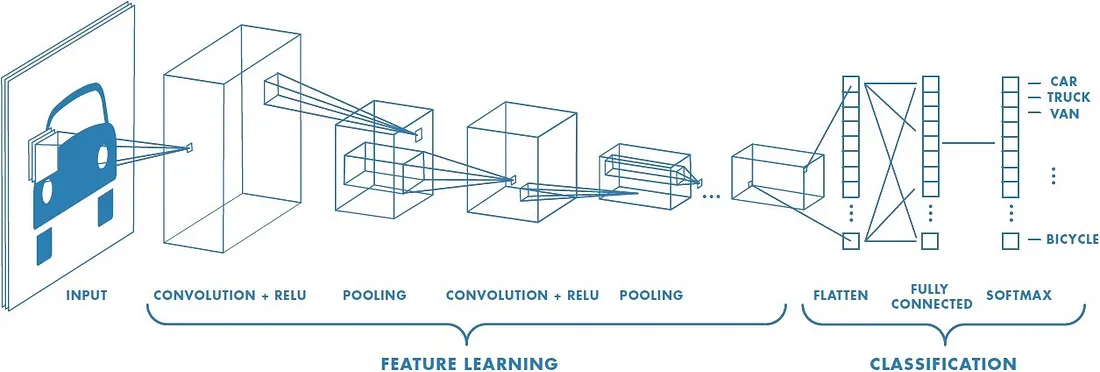
\includegraphics[width=1.0\linewidth]{images/cnn.png}
    \caption{Rede neural convolucional para classificação de imagens \cite{cnn-medium}}
    \label{fig:cnn}
\end{figure}

\section{Modelos de detecção de objetos}

A tarefa de detecção de objetos é um campo desafiador dentro da área mais ampla de visão computacional. Essa tarefa consiste em identificar objetos específicos dentro de uma imagem, incluindo sua classe e localização dentro da imagem. É, portanto, uma tarefa mais complexa que a classificação de imagens, que se preocupa simplesmente em atribuir uma classe à imagem toda, enquanto a detecção de objetos deve extrair da imagem regiões retangulares chamadas \textit{bounding boxes} e atribuir uma classe a cada uma dessas regiões.

Isso permite diversas aplicações como:

\begin{itemize}
    \item Rastrear a movimentação de um objeto ao longo de um vídeo
    \item Verificar quantes instâncias de um dado objeto existem na imagem
    \item Extrair da imagem original uma nova imagem contendo apenas o objeto de interesse
\end{itemize}

A figura \ref{fig:object-detection} exemplifica a tarefa de detecção de objetos em visão computacional.

Os modelos mais comuns de detecção de objetos costumam ser divididos em duas categorias: detectores de duas etapas e detectores de uma etapa \cite{object-detection}. Os modelos de duas etapas primeiro dividem a imagem em regiões candidatas, onde a probabilidade de haver objetos é alta, e posteriormente gera as \textit{bounding boxes} e classifica as regiões. Modelos de duas etapas costumam ser mais precisos, mas o tempo de inferência é mais alto.

Modelos de uma etapa, por outro lado, olham para a imagem inteira e tentam classificar as regiões e gerar as \textit{bounding boxes} diretamente. Esses modelos possuem a vantegem de serem mais rápidos, portanto mais apropriados para aplicações de tempo real.

Como tarefas de detecção de objetos são muito utilizadas em aplicações de tempo real, a velocidade de inferência é uma métrica muito importante na avaliação desse tipo de modelo, além da precisão do resultado. Nessa linha, modelos que colocam grande ênfase na velocidade de inferência ganharam grande tração no campo da detecção de objetos. Um desses modelos (ou família de modelos) é o YOLO, do qual falaremos mais para a frente. 

\begin{figure}[H]
    \centering
    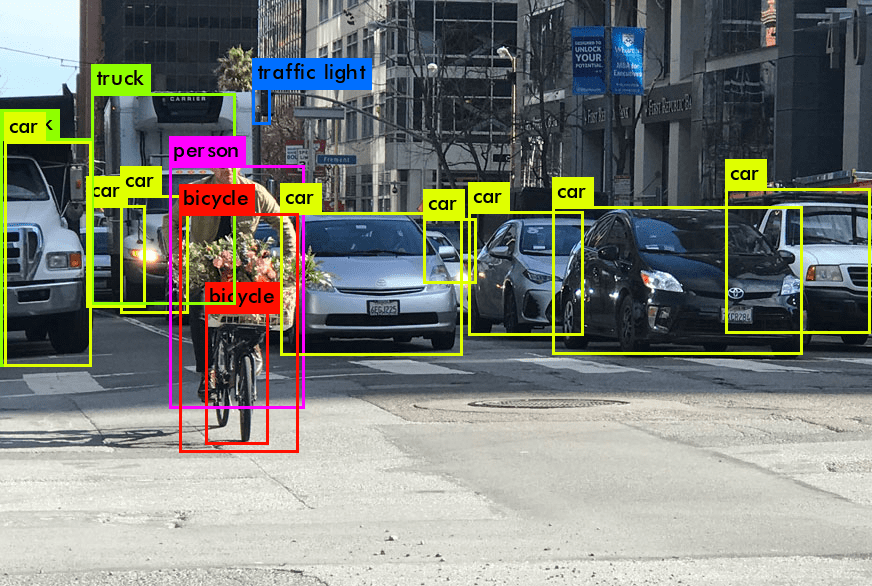
\includegraphics[width=0.6\linewidth]{images/object-detection.png}
    \caption{Exemplo de detecção de objetos}
    \label{fig:object-detection}
\end{figure}

\subsection{Modelos YOLO}

Os modelos da família YOLO (\textit{You Only Look Once}) são modelos muito rápidos de detecção em uma etapa, portanto apropriados para aplicações de tempo real. Quando os modelos YOLO surgiram, apenas modelos de duas etapas eram utilizados para detecção de objetos com redes neurais, mas a inovação proposta com os modelos de uma etapa se mostrou extremamente eficiente e se tornou amplamente utilizada \cite{yolo}.

Modelos YOLO tratam a tarefa de detecção de objetos como uma única tarefa de regressão, diferente dos modelos de duas etapas que se baseiam em uma \textit{pipeline} mais complexa. Ele funciona dividindo a imagem em um grid $SxS$, e cada célula do grid é responsável por detectar os objetos cujo centro está dentro da célula. Cada célula então prevê $B$ \textit{bounding boxes}, sendo que cada \textit{bounding box} é representada por 5 valores: As coordenadas $(x,y)$ do centro relativo à célula, a altura, a largura e a confiança. A confiança representa a IoU (\textit{Intersection over Union}) da \textit{bounding box} prevista com a verdadeira caso haja um objeto na célula. Se não houver objeto a confiança deve ser igual a zero \cite{yolo}.

\begin{equation}
    IoU = \frac{Area \ de \ Interceccao}{Area \ de \ Uniao}
\end{equation}

Cada célula também produz $C$ probabilidades de classe, cada uma representando a probabilidade de aquela célula conter um objeto de uma dada classe.

A figura \ref{fig:yolo-diagram} mostra uma representação do funcionamento da rede YOLO.

\begin{figure}[H]
    \centering
    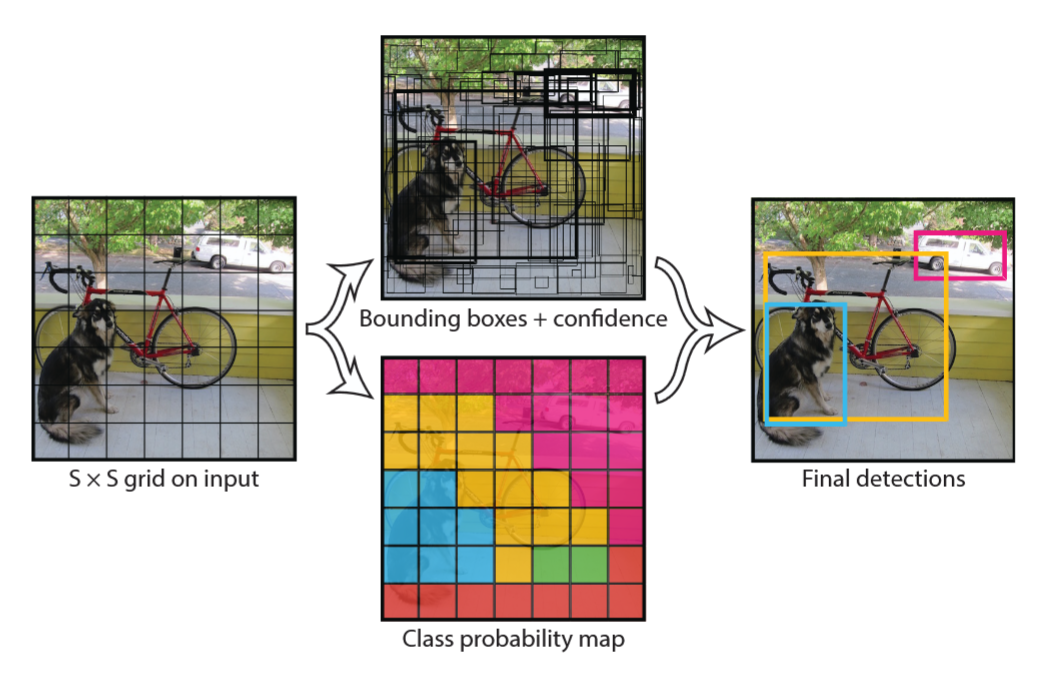
\includegraphics[width=0.6\linewidth]{images/yolo-diagrama.png}
    \caption{Diagrama de funcionamento do modelo YOLO \cite{yolo}}
    \label{fig:yolo-diagram}
\end{figure}

\section{Técnicas de transformação de imagem para visão computacional}

\section{NPU}

\section{Quantização}